\section{Evaluation}

\subsection{RTM Implementation}
We evaluate the proposed approach by implementing a high-performance
application based on the Reverse Time Migration method for seismic
imaging which is used to detect geological structures, based on the
Earth's response to injected acoustic waves. The technique models the
propagation of injected waves using the isotropic acoustic wave
equation \cite{araya2011assessing}:
\begin{align}
\frac{d^2p(r,t)}{dt^2} + {dvv(r)}^2\bigtriangledown^2p(r,t) = f(r,t)
\end{align}

We approximate the differential equation using stencil computation to
perform a fifth-order Taylor expansion in space and first-order Taylor
expansion in time.

We use \MAXC{} to implement the dataflow kernels and aspects to
generate multiple configurations for the design by creating two
kernels that are used to control the memory command read and write
streams (CmdRead, CmdWrite) and the computation kernel (RTM).

To illustrate the potential benefits of our approach we analyse the
results of using the debugging aspect of Section
\ref{sect:asp_debug}. Table \ref{table:loc} compares the number of
lines of code required for the \MAXC{} with aspect design with the
equivalent MaxCompiler implementation showing a reduction in code size
of up to 42\% for the run-time reconfigurable design and a reduction
in the number of API calls (including debug calls) of up to 67\% which
translate to increased productivity.

\begin{table}[!h]
  \renewcommand{\arraystretch}{1.2}
  \centering
  \caption{Code measures for the RTM kernels comparing \MAXC{} and
    MaxCompiler.}
  \label{table:loc}
  \begin{tabular}{c|ccc|cc}
    \hline
    \multirow{2}{*}{\bf{Kernel}} & \bf{Aspect } & \multicolumn{2}{c|}{\bf{\MAXC{}}} & \multicolumn{2}{c}{\bf{MaxCompiler}}                   \\
    \                            & \bf{LOC}     & \bf{LOC}                       & \bf{\# API calls} & \bf{LOC} & \bf{\#API Calls} \\
    \hline \hline
    CmdRead                      & 12           & 26                             &      6         & 59       &      39        \\
    CmdWrite                     & 12           & 28                             &      39        & 79      &       56         \\
    RTM Static                   & 12           & 246                            &     43         & 403     &       175        \\
    RTM RTR                      & 12           & 377                            &     91         & 669     &       275       \\
  \end{tabular}
\end{table}

\subsection{Results}

Results of the design space exploration using the aspect in
Fig.~\ref{fig:aspect-exploration} with variable mantissa illustrate
the trade-offs between accuracy and resource usage
(Fig.~\ref{fig:precision}). We observe irregular, large variations
when decreasing the mantissa from 18 to 16 and 24 to 22 which is the
effect of the backend tools mapping arithmetic to a combination of
both DSPs and LUT/FF elements. The mantissa boundaries at which this
optimisation occurs are platform specific, depending on the
architecture of the DSPs. Hence, automating this optimisation via
aspects and decoupling it from the original source code makes the
application more portable and facilitates discovery of interesting
trade-off opportunities using design space exploration.

\begin{figure}[!h]
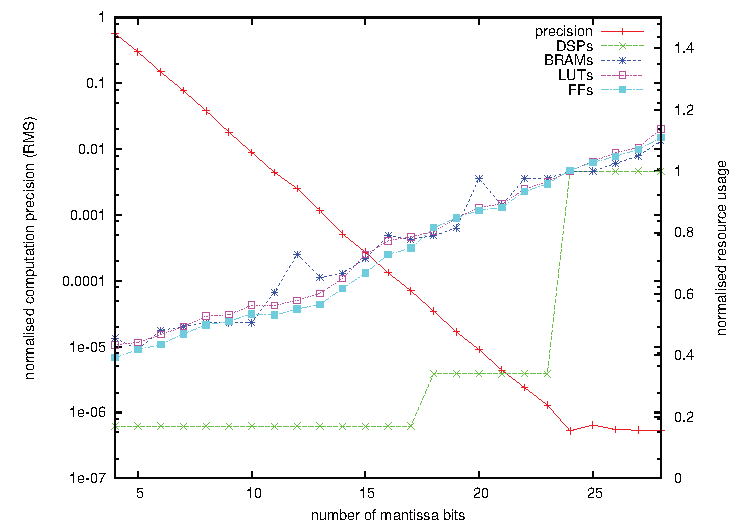
\includegraphics[scale=0.7, trim=0 0 0 0]{figs/pre}
\caption{Exploration of accuracy vs resource usage trade-offs using the aspect
shown in Fig.~\ref{fig:aspect-exploration} with variable mantissa.}
\label{fig:precision}
\end{figure}

The DSP balancing aspect shown in Fig.~\ref{fig:aspect-DSP} allows to
explore the resource trade-offs of implementing arithmetic operations
in either DSPs or LUTs and FFs (Fig.~\ref{fig:arith}) and helps to
avoid over mapping on DSPs for arithmetic intensive applications.

\begin{figure}[!h]
\vspace{0.25cm}
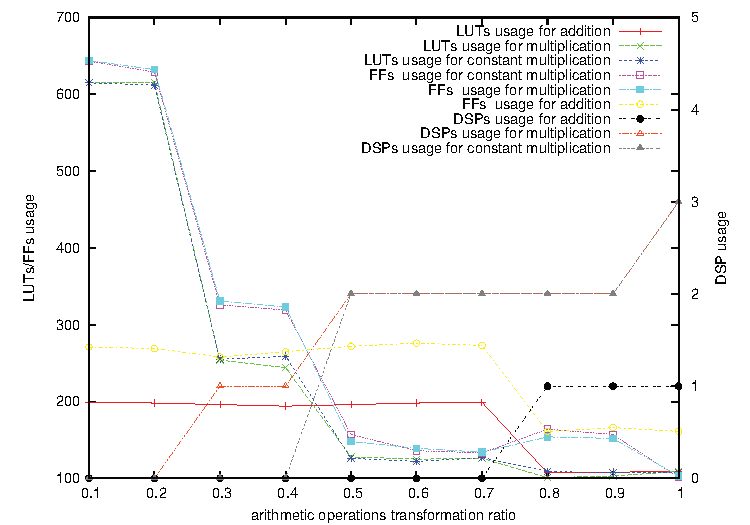
\includegraphics[scale=0.7,trim=0 0 0 0]{figs/arith}
\caption{Exploration of DSP and LUT/FF balancing for functional units
  implementing a single arithmetic operation using the aspect shown
  in Fig.~\ref{fig:aspect-DSP}.}
\label{fig:arith}
\end{figure}


Design space exploration using the aspect in
Fig.~\ref{fig:aspect-exploration} with increasing parallelism level
can be used to investigate design scalability. For example, for the
described RTM implementation, Fig.~\ref{fig:scalability} shows that
performance scales linearly with the number of parallel pipelines and
that significant speedups can be obtained by the \MAXC{} dataflow
design compared to the CPU only implementation. Depending on the
problem size, our approach can be used to achieve a significant
speedup over software only versions which is comparable with the best
published FPGA results for static designs
\cite{Xinyu:Qiwei:Luk:Qiang:Pell:2012}, \cite{araya2011assessing}.


\pgfplotsset{every axis x label/.style={
  at={(0.5,0)},
  below,
  yshift=-5pt}}

\pgfplotsset{every axis y label/.style={
  at={(0,0.5)},
  xshift=-20pt,
  rotate=90}}


\begin{figure}[!h]
  \centering
  \vspace{0.35cm}
  \hspace{-8mm}
  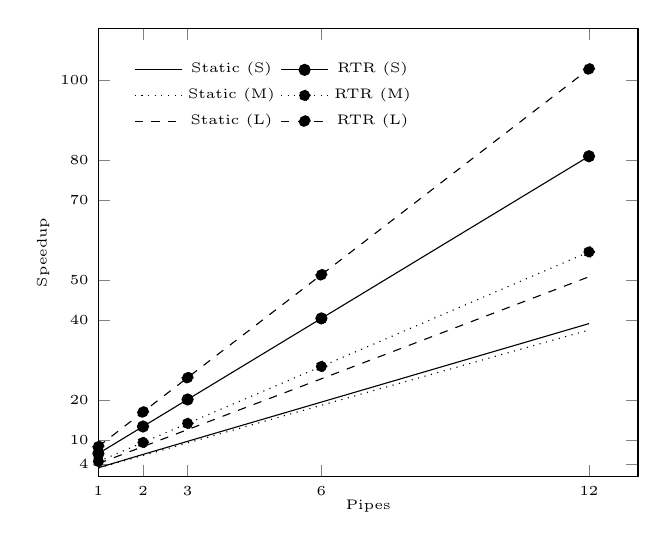
\begin{tikzpicture}[scale=1]
    \selectcolormodel{gray}
    \begin{axis}[
        xmin=1,
        ymin=1,
        %no markers,
        font=\tiny,
        xlabel=Pipes,
        ylabel=Speedup,
        xtick={1,2,3,6,12},
        ytick={4, 10, 20, 40, 50, 70, 80, 100},
        legend columns=2,
        legend entries={
          Static (S),
          RTR (S),
          Static (M),
          RTR (M),
          Static (L),
          RTR (L)},
        legend style={
          draw=none,
          at={(0.05,0.85) },
          anchor=west
        }
      ]

      \addplot[mark=none] coordinates {
        (1, 3.2)
        (2, 6.53)
        (3, 9.8)
        (6, 19.6)
        (12, 39.2)
      };
      \addplot[mark=*] coordinates {
        (1, 6.75)
        (2, 13.5)
        (3, 20.25)
        (6, 40.5)
        (12, 81)
      };
      \addplot[dotted] coordinates {
        (1, 3.13)
        (2, 6.26)
        (3, 9.4)
        (6, 18.8)
        (12, 37.6)
      };
      \addplot[mark=*, dotted] coordinates {
        (1, 4.75)
        (2, 9.51)
        (3, 14.27)
        (6, 28.5)
        (12, 57.1)
      };
      \addplot[mark=none, dashed] coordinates {
        (1, 4.25)
        (2, 8.48)
        (3, 12.725)
        (6, 25.42)
        (12, 50.9)
      };
      \addplot[mark=*, dashed] coordinates {
        (1, 8.5)
        (2, 17.13)
        (3, 25.7)
        (6, 51.4)
        (12, 102.8)
      };
    \end{axis}
  \end{tikzpicture}
  \caption{Scalability of the RTM dataflow design explored using the aspect
shown in Fig.~\ref{fig:aspect-exploration}.}
  \label{fig:scalability}
\end{figure}



Fig.~\ref{fig:scalability} also shows a model of the performance
benefits of using a run-time reconfigurable implementation generated
using the proposed aspect-oriented approach. Two configurations were
created for the RTM \MAXC{} kernel. Since, in our model, during the
first half of the execution time, the backward propagation and imaging
functions are idle, the first configuration requires only half the
resources. Hence, the number of parallel pipelines can be doubled,
halving the execution time of the first configuration. The speedup
obtained is comparable to \cite{Xinyu:Qiwei:Luk:Qiang:Pell:2012}, but
the partitioning and optimisation exploration process is automated via
aspects, which increases developer productivity. The automated process
improves portability of the design, allowing optimisations based on
design space exploration to be carried out on various platforms (hence
subject to varying resource constraints) without manual intervention.
